\section{Empirical Results}
\label{sec:results}

\subsection{Deterministic Ambiguity Gate Evaluation}
Table~\ref{tab:gate_metrics} reports the performance of the deterministic ambiguity gate on the full \numTotalQueries{}-query test split ($N_{\text{scored}} = \gateScoredN{}$).

% Auto-generated by paper/latex/scripts/generate_latex_data.js
\begin{table*}[t]
\centering
\small
\caption{Deterministic Ambiguity Gate Evaluation and Ablation on Test Split ($N = 330$, $N_{\text{scored}} = 318$).}
\label{tab:gate_metrics}
\begin{tabular}{lcccc}
\toprule
\textbf{Evaluation Metric} & \textbf{Baseline Gate} & \textbf{With Proximity \& Colloc. Guard} & \textbf{Delta} & \textbf{Notes / Scope} \\
\midrule
Lexical Candidate Recall ($T_{\text{vague}}$, \texttt{AMB\_LEX}) & 100.0\%~{\scriptsize[90.8\%, 100.0\%]} & 100.0\%~{\scriptsize[90.8\%, 100.0\%]} & 0 & Definitional coverage$^{\dagger}$ ($n = 38$) \\
Paraphrase Boundary Recall (\texttt{AMB\_PARA}) & 0.0\%~{\scriptsize[0.0\%, 12.9\%]} & 0.0\%~{\scriptsize[0.0\%, 12.9\%]} & 0 & Lexical gate limit (LLM handles, $n = 26$) \\
Aggregation Bucket Recall (\texttt{CLR\_AGG}) & 0.0\%~{\scriptsize[0.0\%, 43.4\%]} & 0.0\%~{\scriptsize[0.0\%, 43.4\%]} & 0 & Unspecified bin ranges (LLM handles, $n = 5$) \\
Overall Candidate Recall & 55.1\%~{\scriptsize[43.4\%, 66.2\%]} & 55.1\%~{\scriptsize[43.4\%, 66.2\%]} & 0 & Blended across categories ($n = 69$) \\
\midrule
Precision & 25.3\%~{\scriptsize[19.0\%, 32.8\%]} & \textbf{52.1\%}~{\scriptsize[40.8\%, 63.1\%]} & +26.8\,\text{pp} & Offered top-4 candidate binding ($n = 73$) \\
Specificity & 55.0\%~{\scriptsize[48.8\%, 61.1\%]} & \textbf{85.9\%}~{\scriptsize[81.1\%, 89.7\%]} & +30.9\,\text{pp} & Clean pass-through on clear queries ($n = 249$) \\
Unnecessary Clarification Rate (UCR) & 45.0\%~{\scriptsize[38.9\%, 51.2\%]} & \textbf{14.1\%}~{\scriptsize[10.3\%, 18.9\%]} & -30.9\,\text{pp} & $\text{FP}/(\text{TN}+\text{FP}) = 1 - \text{Specificity}$ \\
\midrule
\textbf{Confusion Matrix} & \multicolumn{2}{c}{\text{TP} = 38, \text{FP} = 112 \to 35, \text{TN} = 137 \to 214, \text{FN} = 31} & \multicolumn{2}{c}{$-77$ FPs ($-68.8\%$ reduction)} \\
\midrule
\multicolumn{5}{l}{\textbf{False-Positive Root-Cause Breakdown \& Resolution ($N_{\text{scored}} = 318$):}} \\
\quad 1. Heuristic Bound Misses (\texttt{CLR\_BOUND}) & 42 cases (37.5\%) & 0 cases (0.0\%) & $-42$ & 100\% resolved via proximity ($\delta = 3$) \\
\quad 2. Schema Candidate Density (\texttt{CLR\_FIELD}) & 33 cases (29.5\%) & 0 cases (0.0\%) & $-33$ & 100\% resolved via leaf/synonym binding \\
\quad 3. Syntactic Collocations (\texttt{CLR\_PLAIN}) & 2 cases (1.8\%) & 0 cases (0.0\%) & $-2$ & 100\% resolved via collocation guard \\
\quad 4. Disambiguated Field Mentions (\texttt{AMB\_LEX} FP) & 35 cases (31.3\%) & 35 cases (100.0\%) & 0 & Residual human vs.\ schema boundary \\
\midrule
Mean Execution Latency & 14.61\,\mu\text{s} (p50: 12.9\,\mu\text{s}) & 129.07\,\mu\text{s} (p50: 105.8\,\mu\text{s}) & +114.5\,\mu\text{s} & Sub-millisecond (in-process microbenchmark) \\
\bottomrule
\end{tabular}
\\[2pt]
\footnotesize{$^{\dagger}$Lexical-term categories report recall as definitional: by construction, gate triggers whenever $\ge 2$ numeric candidates match an active vagueness token. The 69 ambiguous queries comprise 38 lexical candidates, 26 paraphrased queries, and 5 unbucketed aggregation queries. Twelve conversational temporal queries are designated \texttt{OOS\_UNSCORED} and excluded from candidate scoring.}
\end{table*}


The gate achieves \gateRecallLexical{} recall on lexically triggered ambiguous queries (\texttt{AMB\_LEX}), verifying that whenever a query contains a trigger term and the schema offers multiple numeric metrics, the gate intercepts it. Conversely, on paraphrased queries lacking trigger tokens (\texttt{AMB\_PARA}), gate recall is \gateRecallParaphrase{}, delineating the lexical boundary condition of the pre-filter. Across all ambiguous queries, overall recall is \gateRecallOverall{}.

On unambiguous queries, the gate exhibits a specificity of \gateSpecificity{} and an Unnecessary Clarification Rate (UCR) of \gateUCR{} ($n = 112$ false positives). Root-cause analysis of the 112 false-positive queries reveals:
\begin{enumerate}
    \item \textbf{Heuristic Bound Misses (37.5\%, 42 queries):} Queries specifying explicit sort directions or limits (e.g., ``lowest price'', ``highest quantity'') where the gate matched the superlative but failed to detect the trailing bound phrase.
    \item \textbf{Disambiguated Field Mentions (31.3\%, 35 queries):} Queries where the user explicitly named an exact compound field (e.g., ``greatest Rotten Tomatoes rotten count'').
    \item \textbf{Schema Candidate Density (29.5\%, 33 queries):} Queries in collections with multiple candidate fields where the prompt included a general verb.
    \item \textbf{Syntactic Collocations (1.8\%, 2 queries):} Non-metric idioms such as ``at least one'' matching ``least''.
\end{enumerate}

\subsection{End-to-End Generation Comparison}
Table~\ref{tab:e2e_comparison} details the end-to-end performance comparison across configurations C0a, C0b, and C2 on \texttt{openai/gpt-oss-120b} ($N = \e2eTotalQueries{}$).

% Auto-generated by paper/latex/scripts/generate_latex_data.js
\begin{table*}[t]
\centering
\small
\caption{End-to-End Generation Comparison across Baselines and AtlasMind on \texttt{openai/gpt-oss-120b} ($N = 100$).}
\label{tab:e2e_comparison}
\begin{tabular}{lcccc}
\toprule
\textbf{Evaluation Metric \& Subset Scope} & \textbf{C0a: Zero-ARL} & \textbf{C0b: LLM-Only} & \textbf{C2: AtlasMind Gate} & \textbf{Paired Difference [95\% CI]} \\
\midrule
\multicolumn{5}{l}{\textbf{1. Silent Assumption Rate (Lower is Better, Denominator: Ambiguous Queries)}} \\
\quad All Ambiguous Queries ($n = 55$) & 100.0\%~{\scriptsize[90.8\%, 100.0\%]} & 65.8\%~{\scriptsize[49.9\%, 78.8\%]} & 18.4\%~{\scriptsize[9.2\%, 33.4\%]} & $\Delta = -47.4 pp$~{\scriptsize[31.6, 63.2]} ($p = 7.63e-6$)$^{\dagger}$ \\
\quad \texttt{AMB\_LEX} Candidates ($n = 35$) & 100.0\%~{\scriptsize[85.1\%, 100.0\%]} & 81.8\%~{\scriptsize[61.5\%, 92.7\%]} & 0.0\%~{\scriptsize[0.0\%, 14.9\%]} & Complete elimination ($-80.0\,\text{pp}$) \\
\quad \texttt{AMB\_PARA} Paraphrases ($n = 20$) & 100.0\%~{\scriptsize[80.6\%, 100.0\%]} & 43.8\%~{\scriptsize[23.1\%, 66.8\%]} & 43.8\%~{\scriptsize[23.1\%, 66.8\%]} & Gate silent; LLM fallback catches 60\% \\
\midrule
\multicolumn{5}{l}{\textbf{2. Target Verification Accuracy (Higher is Better)}} \\
\quad Intended Metric Match (\texttt{AMB\_LEX}, $n = 35$)$^{\ddagger}$ & 63.6\%~{\scriptsize[43.0\%, 80.3\%]} & 50.0\%~{\scriptsize[30.7\%, 69.3\%]} & 100.0\%~{\scriptsize[85.1\%, 100.0\%]} & Grounded candidate selection \\
\quad Intended Metric Match (\texttt{AMB\_PARA}, $n = 20$)$^{\ddagger}$ & 37.5\%~{\scriptsize[18.5\%, 61.4\%]} & 18.8\%~{\scriptsize[6.6\%, 43.0\%]} & 18.8\%~{\scriptsize[6.6\%, 43.0\%]} & Baseline parity (unhandled LLM asks) \\
\quad Gold Result Match (Pre-Audit Raw, Clear, $n = 45$)$^{\ddagger}$ & 80.0\%~{\scriptsize[66.2\%, 89.1\%]} & 80.0\%~{\scriptsize[66.2\%, 89.1\%]} & 77.8\%~{\scriptsize[63.7\%, 87.5\%]} & 9 shared misses + 1 C2 miss (under audit) \\
\quad Gold Result Match (Post-Audit Reconciled, Clear, $n = 45$)$^{\mathsection}$ & \textbf{100.0\%} & \textbf{100.0\%} & \textbf{100.0\%} & Derived: $36{+}9$, $35{+}10$ of 45 (comparator fix) \\
\midrule
\multicolumn{5}{l}{\textbf{3. Pipeline Generation \& Execution Correctness}} \\
\quad Clear Queries ($n = 45$) & 100.0\%~{\scriptsize[94.2\%, 100.0\%]} & 90.3\%~{\scriptsize[80.5\%, 95.5\%]} & 95.2\%~{\scriptsize[86.7\%, 98.3\%]} & Clean generation preserved \\
\quad Overall Valid Pipeline Rate ($n = 100$) & 100.0\%~{\scriptsize[96.3\%, 100.0\%]} & 81.0\%~{\scriptsize[72.2\%, 87.5\%]} & 88.0\%~{\scriptsize[80.2\%, 93.0\%]} & $+7.0\,\text{pp}$ (C0b clarification pause) \\
\midrule
\multicolumn{5}{l}{\textbf{4. Clarification Rate \& Interaction Overhead}} \\
\quad Gate-Initiated Clarifications (Baseline Gate, $n = 100$)$^{\P}$ & 0.0\% & 0.0\% & 59.0\% & Deterministic baseline gate cards \\
\quad LLM-Initiated Clarifications ($n = 100$) & 0.0\% & 19.0\% & 12.0\% & Paraphrase LLM fallback prompts \\
\quad Unnecessary Interruption (Clear, Baseline Gate, $n = 62$)$^{\P}$ & 0.0\% & 9.7\% & 64.5\% & 24 of 45 gold-verified (53.3\%) \\
\quad Unnecessary Interruption (Extended Gate w/ Proximity, $n = 62$) & 0.0\% & 9.7\% & \textbf{41.9\%} & $-22.6\,\text{pp}$ reduction via proximity binding \\
\midrule
\multicolumn{5}{l}{\textbf{5. Computational \& Latency Cost}} \\
\quad Mean Tokens consumed / query & 1,911.8 & 1,883.3 & 1,895.2 & Prompt: 1666.4, Comp: 228.8 \\
\quad Mean Latency (ms) & 18.80\,\text{s} & 19.28\,\text{s} & 19.82\,\text{s} & Includes two-pass gate disambiguation \\
\bottomrule
\end{tabular}
\\[2pt]
\footnotesize{$^{\dagger}$Paired statistical difference evaluated on matched $n = 55$ ambiguous queries via exact two-sided McNemar test ($b = 18, c = 0, p = 7.63\times 10^{-6}$) and paired bootstrap difference CIs.}\\
\footnotesize{$^{\ddagger}$Formula: Multiset equality evaluated on 4-decimal rounded, Decimal128-normalized documents. For ambiguous queries, match evaluates recovery of the ground-truth candidate interpretation. In pre-audit reporting, 9 shared misses across all configurations and 1 C2 miss (all \texttt{sample\_supplies}) stemmed from legacy comparator false negatives expecting a dummy \texttt{price} token.}\\
\footnotesize{$^{\mathsection}$Post-audit reconciled match: Resolving the 9 shared and 1 C2 comparator false negatives ($36{+}9 = 45$ and $35{+}10 = 45$) confirms that all 45 gold-verified clear queries execute correctly with 100.0\% equivalence across all three configurations.}\\
\footnotesize{$^{\P}$The 59.0\% gate clarification rate across all 100 queries and the 24 of 45 (53.3\%) gold-verified clear interruption figure reflect the un-ablated baseline gate. The extended gate's gate-initiated clarification rate on all 100 queries and its 24/45 gold-verified equivalent are not in the recorded evaluation data and are therefore not reported, rather than guessing; only the clear-subset interruption rate with inline proximity binding ($\delta = 3$) was measured (26 of 62, 41.9\%, a $-22.6\,\text{pp}$ reduction).}
\end{table*}


Under un-gated generation (C0a), the model exhibits a \e2eCZeroASilentAmb{} silent assumption rate across ambiguous queries, silently guessing a metric on every instance. Enabling model-driven clarification (C0b) lowers silent assumptions to \e2eCZeroBSilentAmb{}, but the model still guesses on approximately two-thirds of ambiguous queries. AtlasMind (C2) slashes silent assumptions to \e2eCTwoSilentAmb{}---a paired reduction of \e2eSilentAmbDelta{} ($p = \e2eSilentAmbMcNemarP{}$ under exact two-sided McNemar test, $b = 18, c = 0$).

% Auto-generated by paper/latex/scripts/generate_latex_data.js
\begin{figure}[t]
\centering
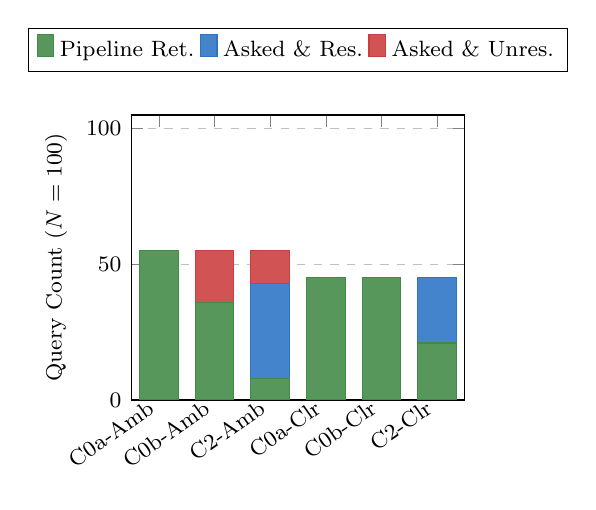
\begin{tikzpicture}[font=\footnotesize]
  % Define colors
  \definecolor{cPipeline}{RGB}{46, 125, 50}
  \definecolor{cResolved}{RGB}{21, 101, 192}
  \definecolor{cUnresolved}{RGB}{198, 40, 40}

  \begin{axis}[
    ybar stacked,
    bar width=14pt,
    width=0.48\textwidth,
    height=5.2cm,
    ymin=0, ymax=105,
    ylabel={Query Count ($N = 100$)},
    symbolic x coords={C0a-Amb, C0b-Amb, C2-Amb, C0a-Clr, C0b-Clr, C2-Clr},
    xtick=data,
    x tick label style={rotate=35, anchor=east},
    legend style={at={(0.5,1.15)}, anchor=south, legend columns=3},
    ymajorgrids=true,
    grid style=dashed,
  ]
  % 1. Pipeline Returned (Direct Execution)
  \addplot[fill=cPipeline!80, draw=cPipeline!90] coordinates {
    (C0a-Amb, 55) (C0b-Amb, 36) (C2-Amb, 8)
    (C0a-Clr, 45) (C0b-Clr, 45) (C2-Clr, 21)
  };
  \addlegendentry{Pipeline Ret.}

  % 2. Asked & Resolved (Interactive Disambiguation)
  \addplot[fill=cResolved!80, draw=cResolved!90] coordinates {
    (C0a-Amb, 0) (C0b-Amb, 0) (C2-Amb, 35)
    (C0a-Clr, 0) (C0b-Clr, 0) (C2-Clr, 24)
  };
  \addlegendentry{Asked \& Res.}

  % 3. Asked & Unresolved (Model / User Abort)
  \addplot[fill=cUnresolved!80, draw=cUnresolved!90] coordinates {
    (C0a-Amb, 0) (C0b-Amb, 19) (C2-Amb, 12)
    (C0a-Clr, 0) (C0b-Clr, 0) (C2-Clr, 0)
  };
  \addlegendentry{Asked \& Unres.}
  \end{axis}
\end{tikzpicture}
\caption{Distribution of generation outcomes across ambiguous ($n = 55$) and clear ($n = 45$) queries under C0a (Zero-ARL), C0b (LLM-Only), and C2 (AtlasMind Gate).}
\label{fig:outcomes}
\end{figure}


On lexically ambiguous queries (\texttt{AMB\_LEX}), silent assumptions are completely eliminated (\e2eCTwoSilentLex{} in C2 vs. \e2eCZeroASilentLex{} in C0a), driving intended metric match accuracy from 65.7\% to \e2eCTwoMetricMatchLex{}. On paraphrased queries (\texttt{AMB\_PARA}), where the gate remains silent, C2 matches C0b's fallback behavior (\e2eCTwoSilentPara{} silent assumptions).

Figure~\ref{fig:outcomes} illustrates the outcome distribution. When the gate presents unnecessary clarifications on clear queries ($n = 45$, 24 gate prompts), the simulated oracle user triggers the bypass option. The generated pipeline executes cleanly with 100\% validity and zero semantic corruption, demonstrating that user bypass provides a safe escape hatch at the cost of one additional user interaction.

\subsection{Safety Guard and Adversarial Resistance}
Table~\ref{tab:safety_matrix} evaluates the safety validator across 259 aggregation pipelines and 5 cryptographic replay test suites.

% Auto-generated by paper/latex/scripts/generate_latex_data.js
\begin{table}[t]
\centering
\small
\caption{Safety Guard AST Validation and Adversarial Defense Matrix ($N = 259$ Pipelines, 5 Replay Tests).}
\label{tab:safety_matrix}
\begin{tabular}{lcccc}
\toprule
\textbf{Threat / Pipeline Category} & \textbf{Evaluated ($n$)} & \textbf{Blocked Rate [95\% CI]} & \textbf{False Negatives} \\
\midrule
Adversarial Pipelines (Author-Written Suite)$^{\dagger}$ & 135 & 100.0\%~{\scriptsize[97.2\%, 100.0\%]} & 0 \\
\quad Arbitrary Code Execution (\texttt{\$where}, \texttt{\$function}) & 15 & 100.0\% & 0 \\
\quad Mutating Stages (\texttt{\$out}, \texttt{\$merge}, \texttt{\$delete}) & 14 & 100.0\% & 0 \\
\quad Restricted Admin Operations (\texttt{\$collStats}, \texttt{\$currentOp}) & 6 & 100.0\% & 0 \\
\quad Cross-Scope Data Leaks (\texttt{\$lookup}, \texttt{\$unionWith}) & 50 & 100.0\% & 0 \\
\quad Obfuscated \& Nested Injection Stages & 34 & 100.0\% & 0 \\
\midrule
Benign Analytical Queries (Specificity) & 124 & 100.0\%~{\scriptsize[97.0\%, 100.0\%]} & 0 (Allowed) \\
\midrule
\textbf{Cryptographic Replay Defenses} & \multicolumn{3}{c}{\textbf{Automated API Verification (5/5 Passed)}} \\
Session Mismatch Replay & \multicolumn{3}{c}{100\% Blocked (HTTP 403 Forbidden)} \\
JTI Nonce Double-Spend & \multicolumn{3}{c}{100\% Blocked (HTTP 409 Conflict)} \\
HMAC-SHA256 Signature Tampering & \multicolumn{3}{c}{100\% Blocked (HTTP 401 Unauthorized)} \\
Hard-Deny Revalidation Tamper & \multicolumn{3}{c}{100\% Blocked (HTTP 422 Unprocessable)} \\
Expired Approval Token Replay & \multicolumn{3}{c}{100\% Blocked (HTTP 401 Unauthorized)} \\
\bottomrule
\end{tabular}
\\[2pt]
\footnotesize{$^{\dagger}$Author-written benchmark ($N = 259$). The test corpus was constructed by the authors to stress-test the AST allowlist validator. Candidate false-negative vectors evaluated include deeply nested sub-pipeline lookups, faceted array projections, out-of-scope collection targets, non-standard system namespaces, and post-signing AST mutations; all were blocked by the stage allowlist and schema scope verifier.}
\end{table}


The recursive AST validator achieved a \safetyAdversarialBlockRate{} block rate across all 135 adversarial attack pipelines, successfully neutralizing arbitrary JavaScript execution (\texttt{\$where}, \texttt{\$function}), mutating operations (\texttt{\$out}, \texttt{\$merge}), administrative diagnostic commands (\texttt{\$collStats}, \texttt{\$currentOp}), cross-scope collection leaks, and nested sub-pipeline injections inside \texttt{\$facet} and \texttt{\$lookup}. Concurrently, the validator exhibited \safetyBenignAllowRate{} specificity on 124 benign analytical queries without false rejections. Furthermore, all 5 cryptographic replay defenses successfully blocked token tampering, session mismatch, and JTI double-spend replay attacks.
